\documentclass[aspectratio=169,11pt]{beamer}
\usetheme{default}
\usecolortheme{seahorse}
\setbeamertemplate{navigation symbols}{}
\setbeamertemplate{footline}[frame number]
\usepackage{amsmath,amssymb}
\usepackage{graphicx}
\usepackage{booktabs}

\graphicspath{{../figures/}}

% AUTO-GENERATED from results/results.json -- do not edit
\newcommand{\RefYA}{0.7158271}
\newcommand{\RefYB}{9.1855\times10^{-6}}
\newcommand{\RefYC}{0.2841637}
\newcommand{\RefDefect}{2.9\times10^{-15}}
\newcommand{\OrdEulerRob}{1.00}
\newcommand{\OrdImplRob}{1.00}
\newcommand{\OrdRKRob}{4.35}
\newcommand{\StiffOne}{3.03\times10^{3}}
\newcommand{\StiffTwo}{5.42\times10^{3}}
\newcommand{\StiffForty}{1.584\times10^{5}}
\newcommand{\LamMaxForty}{3.39\times10^{3}}
\newcommand{\HBoundEuler}{0.00059}
\newcommand{\HBoundRK}{0.00083}
\newcommand{\HCritEmp}{0.0006}
\newcommand{\SweepTableBody}{
$0.0003$ & stable (bounded) & $0$ \\
$0.0004$ & stable (bounded) & $0$ \\
$0.0005$ & stable (bounded) & $0$ \\
$0.00055$ & stable (bounded) & $0$ \\
$0.0006$ & bounded, \textbf{negative} & $-4.9\times10^{-6}$ \\
$0.0007$ & \textbf{blow-up} & -- \\
$0.0008$ & \textbf{blow-up} & -- \\
$0.001$ & \textbf{blow-up} & -- \\
}
\newcommand{\MatchedTableBody}{
Explicit Euler & $10^{2}$ & $0.00053$ & $1.9\times10^{-6}$ & 75,395 & 0.50\,s\,\,(stab.-pinned) \\
Explicit Euler & $10^{3}$ & $0.00053$ & $1.9\times10^{-6}$ & 75,395 & 0.51\,s\,\,(stab.-pinned) \\
Explicit Euler & $10^{4}$ & $0.00053$ & $1.9\times10^{-6}$ & 75,395 & 0.47\,s\,\,(stab.-pinned) \\
RK4 & $10^{2}$ & $0.00063$ & $2.6\times10^{-12}$ & 252,060 & 2.11\,s\,\,(stab.-pinned) \\
RK4 & $10^{3}$ & $0.00063$ & $2.6\times10^{-12}$ & 252,060 & 2.50\,s\,\,(stab.-pinned) \\
RK4 & $10^{4}$ & $0.00063$ & $2.6\times10^{-12}$ & 252,060 & 2.07\,s\,\,(stab.-pinned) \\
Implicit Euler & $10^{2}$ & $2$ & $0.0065$ & 93 & 0.01\,s \\
Implicit Euler & $10^{3}$ & $0.3$ & $0.001$ & 421 & 0.03\,s \\
Implicit Euler & $10^{4}$ & $0.029$ & $0.0001$ & 3,505 & 0.22\,s \\
}
\newcommand{\AdaptiveTableBody}{
$10^{4}$ & $1.2\times10^{-6}$ & 20,604 & 8,766 & 323,070 & 3.31\,s \\
$10^{5}$ & $6.1\times10^{-7}$ & 20,636 & 8,856 & 324,412 & 4.49\,s \\
$10^{6}$ & $1.2\times10^{-6}$ & 20,758 & 9,126 & 328,724 & 4.38\,s \\
}


\newcommand{\takeaway}[1]{\vskip2pt\begin{beamercolorbox}[rounded=true,leftskip=4pt]{block body}\small\textbf{Takeaway:} #1\end{beamercolorbox}}

\title{Stiffness in the Robertson Chemical Kinetics System}
\subtitle{What explicit methods pay --- what implicit methods buy}
\author{Team of 3 \\ Numerical Analysis of ODEs and PDEs --- Project 1}
\date{\today}

\begin{document}

\begin{frame}
\titlepage
\small One question: \emph{how does stiffness translate into a practical step-size
restriction for explicit methods --- and what does an implicit method pay for the
same accuracy?}
\end{frame}

\begin{frame}{The problem: Robertson chemical kinetics}
\[
\begin{aligned}
y_1' &= -0.04\,y_1 + 10^4 y_2 y_3\\
y_2' &= 0.04\,y_1 - 10^4 y_2 y_3 - 3\times10^7 y_2^2\\
y_3' &= 3\times10^7 y_2^2
\end{aligned}
\qquad y(0)=[1,0,0]^{\mathsf T},\quad 0\le t\le 40
\]
\begin{itemize}
\item Rate constants span $10^8$; the state spans $10^5$ ($y_2\sim10^{-5}$ vs $y_1\sim1$)
\item Invariant plane $y_1+y_2+y_3=1$ $\Rightarrow$ structural zero eigenvalue
\item Stiffness ratio over the two nonzero eigenvalues grows to $\StiffForty$ at $t=40$
\end{itemize}
\takeaway{a benchmark designed so that explicit methods fail for a measurable, quantitative reason.}
\end{frame}

\begin{frame}{What we built --- and how we trust it}
\begin{columns}
\column{0.52\textwidth}
\textbf{From scratch:} explicit Euler, RK4, implicit Euler + Newton, adaptive
step-doubling RK4 --- swappable $f$, built-in cost counters.
\medskip

\textbf{Our own oracle:} scipy Radau, $\mathrm{rtol}=10^{-12}$, tightened
$\sim45\times$; digits that survive the repeat are the only ones we quote.
\column{0.44\textwidth}
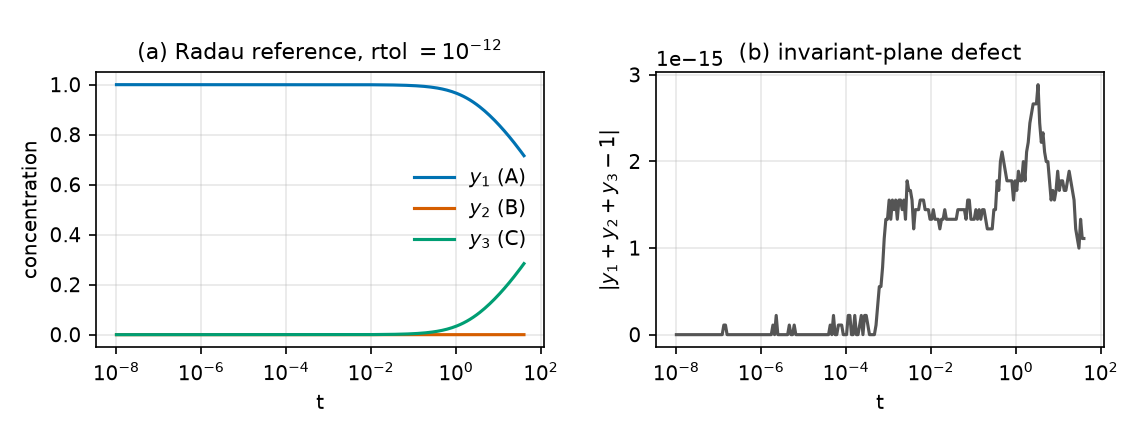
\includegraphics[width=\textwidth]{fig1_reference.png}
\end{columns}
\takeaway{$y(40)=(\RefYA,\ \RefYB,\ \RefYC)$ to 15 digits; invariant defect $\RefDefect$; Problem Pack check value reproduced.}
\end{frame}

\begin{frame}{Orders are verified, not assumed}
\begin{columns}
\column{0.55\textwidth}
Observed order (slope of $\log err$ vs $\log h$) on the stable window
$0\le t\le0.5$:
\begin{tabular}{lccc}
\toprule
 & Euler & RK4 & Impl.\\
\midrule
scalar & 1.00 & 4$^*$ & 1.00\\
Robertson & \OrdEulerRob & \OrdRKRob & \OrdImplRob\\
\bottomrule
\end{tabular}

\small $^*$ round-off floor flattens the tail.
\column{0.42\textwidth}
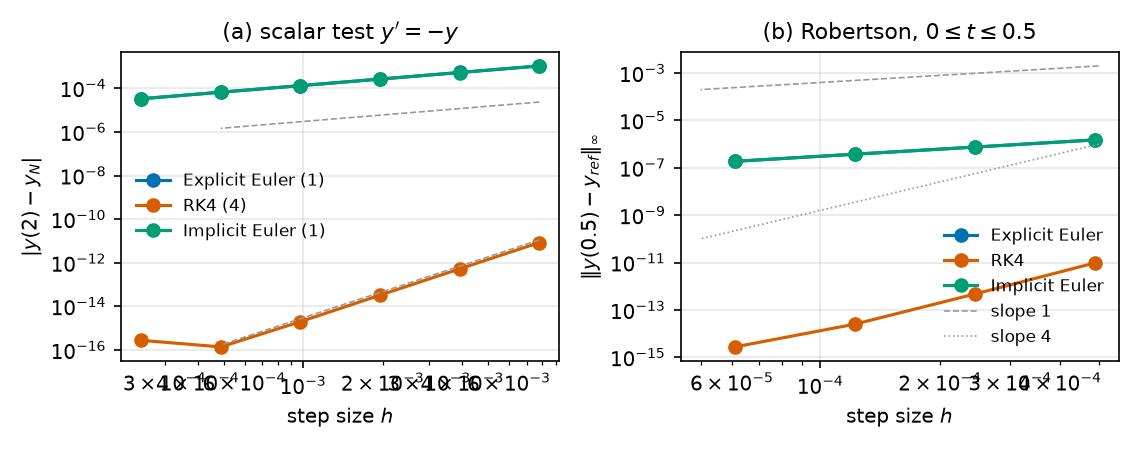
\includegraphics[width=\textwidth]{fig2_convergence.png}
\end{columns}
\takeaway{Euler and implicit Euler have the same order-1 constant --- they differ in stability, not per-step accuracy.}
\end{frame}

\begin{frame}{Stability regions: hard ceilings for explicit methods}
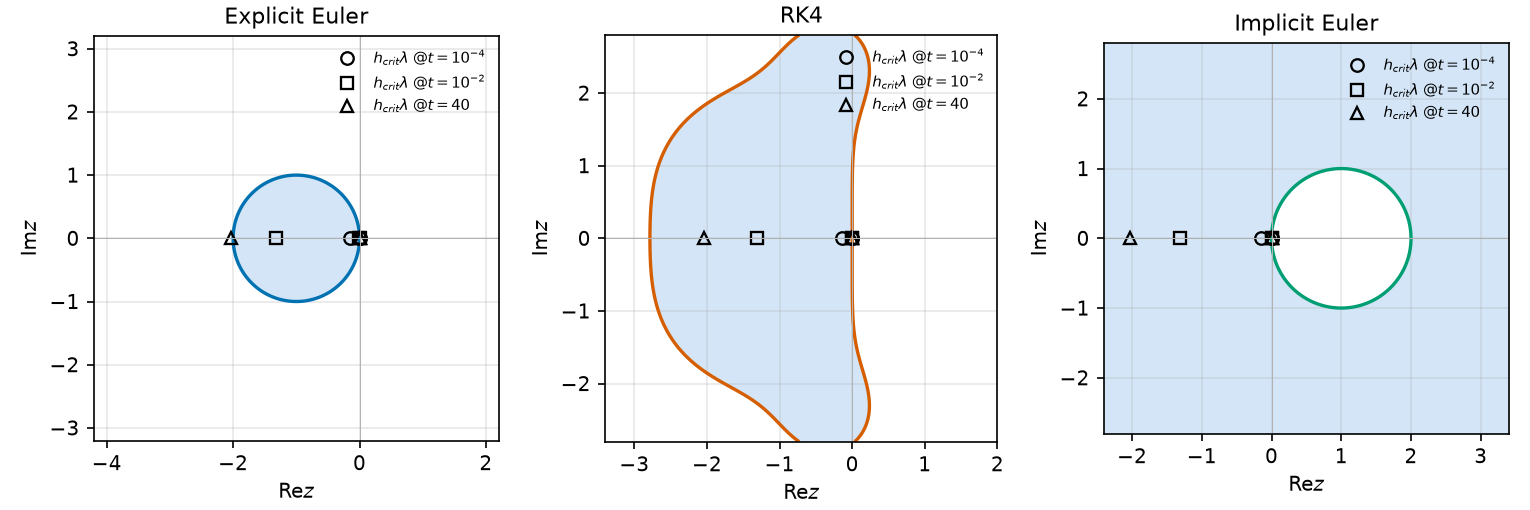
\includegraphics[width=\textwidth]{fig3_stability_regions.png}
\medskip
\centerline{$h_{\text{Euler}}<2/|\lambda|_{\max}=\HBoundEuler$,\qquad
$h_{\text{RK4}}<2.8/|\lambda|_{\max}=\HBoundRK$, implicit Euler $A$-stable.}
\takeaway{the frozen-Jacobian eigenvalue at $t=40$ sets a hard step ceiling --- and we test it empirically next.}
\end{frame}

\begin{frame}{Stiffness grows along the trajectory}
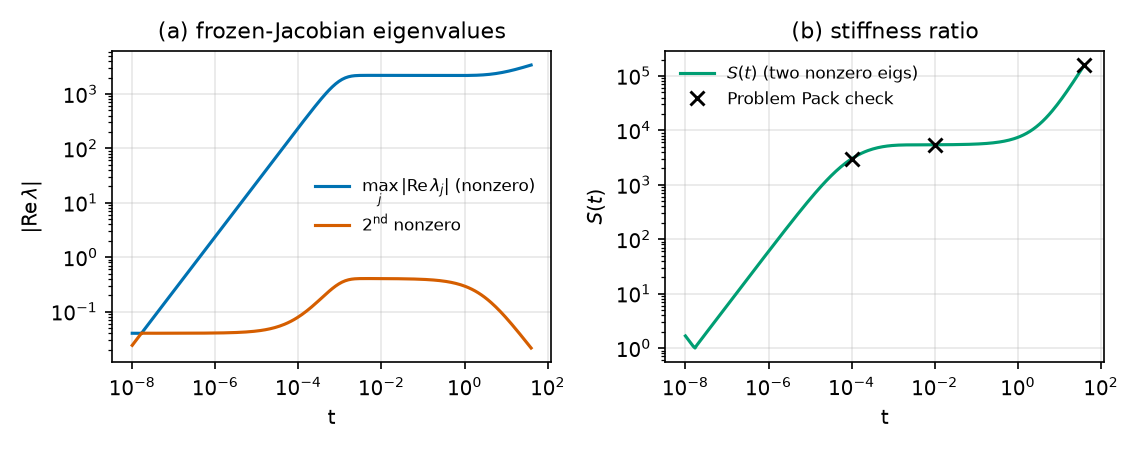
\includegraphics[width=\textwidth]{fig7_stiffness.png}
\takeaway{$S(t)$: $\StiffOne\to\StiffTwo\to\StiffForty$ at $t=10^{-4},10^{-2},40$ --- matches the Problem Pack check values.}
\end{frame}

\begin{frame}{Explicit failure: physics fails before arithmetic}
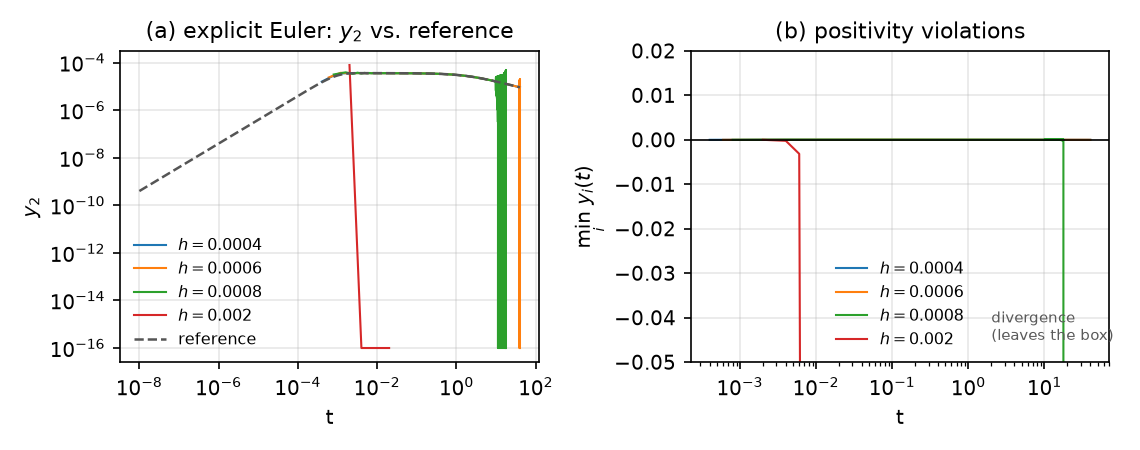
\includegraphics[width=\textwidth]{fig4_explicit_failure.png}
\medskip
measured threshold $h_{\text{crit}}=\HCritEmp$ vs.\ prediction $\HBoundEuler$ (2\% error).
\takeaway{positivity is lost (bounded but non-physical) \emph{before} blow-up --- ``did not explode'' is not ``is right''.}
\end{frame}

\begin{frame}{Cost vs.\ accuracy at matched error}
\begin{center}
\small
\begin{tabular}{llrrrl}
\toprule
Method & Target & $h$ & error & nfev & wall\\
\midrule
\MatchedTableBody
\bottomrule
\end{tabular}
\end{center}
\takeaway{implicit Euler wins by $810\times/179\times/21\times$ at targets $10^{-2}/10^{-3}/10^{-4}$ --- explicit methods are pinned at their stability limit and cannot loosen up.}
\end{frame}

\begin{frame}{RK4's order is wasted on the stiff interval}
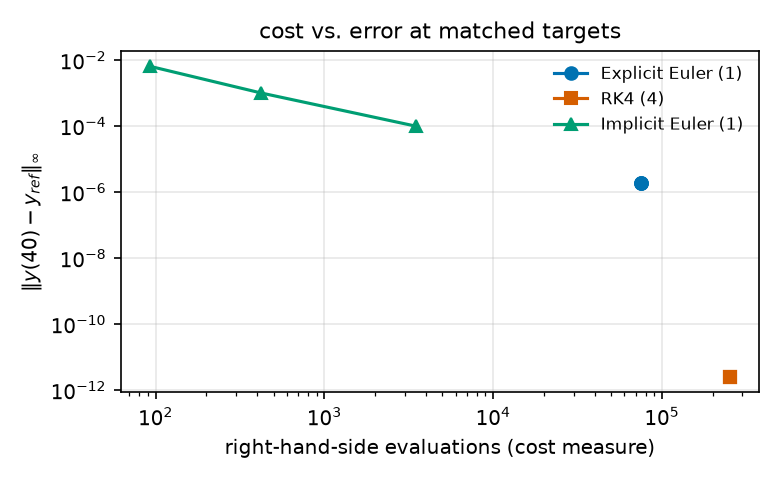
\includegraphics[width=0.55\textwidth]{fig5_matched_cost.png}
\begin{itemize}
\item RK4: error $2.6\times10^{-12}$ \emph{always} --- its $h$ is pinned at the stability limit for every target
\item highest nfev, accuracy far beyond anything requested
\end{itemize}
\takeaway{on a stiff interval the binding constraint is stability, not accuracy --- order alone does not win.}
\end{frame}

\begin{frame}{Adaptive RK4: accuracy responds --- stability does not}
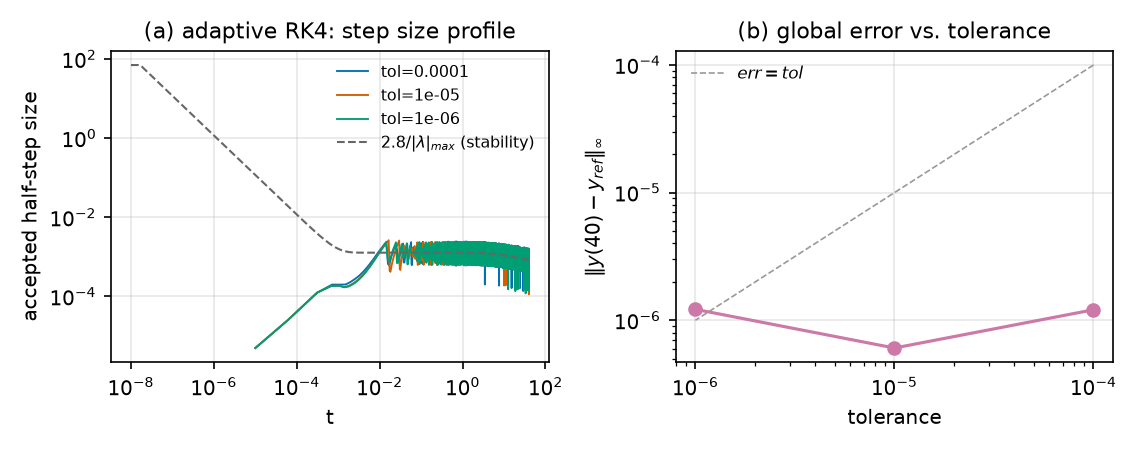
\includegraphics[width=\textwidth]{fig6_adaptive.png}
\medskip
step size adapts over 3 orders of magnitude; controller tracks the
$2.8/|\lambda|_{\max}$ envelope from below.
\takeaway{error follows the tolerance down to $\sim10^{-6}$ and then \emph{plateaus}: adaptivity buys accuracy, not stability.}
\end{frame}

\begin{frame}{Conclusions}
\begin{enumerate}
\item frozen-Jacobian prediction verified to $\sim2\%$ ($\HCritEmp$ vs $\HBoundEuler$)
\item at matched error, implicit Euler wins by $21\times$--$810\times$ (nfev) on $[0,40]$
\item RK4's order 4 is irrelevant here --- stability pins its step
\item adaptive controller: error plateaus at the stability ceiling
\item diagnostics fail in order: positivity $\to$ stability $\to$ (conservation survives)
\end{enumerate}
\takeaway{stiffness is a stability story --- measure it, don't assume it.}
\end{frame}

\begin{frame}{Reproducibility}
\begin{itemize}
\item \texttt{python code/run\_all.py} regenerates every figure and every number
      (\texttt{results/results.json} $\to$ \texttt{numbers.tex} $\to$ report)
\item \texttt{requirements.txt}: numpy, scipy, matplotlib --- no other dependencies
\item AI use documented in the AI Transparency Log (report App.~B);
      ICS backed by git history (App.~A)
\end{itemize}
\vfill
\small Repository: \texttt{github.com/\dots/robertson-stiff-ode} --- all team members can explain and modify every part (viva-ready).
\end{frame}

\end{document}
